\documentclass[onecolumn]{article}
%\usepackage{url}
%\usepackage{algorithmic}
\usepackage[a4paper]{geometry}
\usepackage{datetime}
\usepackage[margin=2em, font=normalsize,labelfont=it]{caption}
\usepackage{graphicx}
\usepackage{mathpazo} % use palatino
\usepackage[scaled]{helvet} % helvetica
\usepackage{microtype}
\usepackage{amsmath}
\usepackage{subfigure}

% Letterspacing macros
\newcommand{\spacecaps}[1]{\textls[200]{\MakeUppercase{#1}}}
\newcommand{\spacesc}[1]{\textls[50]{\textsc{\MakeLowercase{#1}}}}

\title{\spacecaps{World Happiness Report}\\ \normalsize \spacesc{Data Mining Final Project} }

\author{Kıymet Deren Toy - Görkem Savran\\kiymetderentoy@posta.mu.edu.tr - gorkemsavran@posta.mu.edu.tr}
%\date{\today\\\currenttime}
\date{\today}
\usepackage[utf8]{inputenc}
\usepackage[english]{babel}

\usepackage{hyperref}
\hypersetup{
    colorlinks=true,
    linkcolor=blue,
    filecolor=magenta,      
    urlcolor=cyan,
}

\urlstyle{same}



\begin{document}

\maketitle
\fontfamily{qag}\selectfont 
\section{Introduction}
First of all, our data set includes the names of countries, their happiness scores and the factors 
that affect this score. The source of our data is 
\href{https://www.kaggle.com/unsdsn/world-happiness?select=2019.csv}{Kaggle} and we have 
data for 5 
different years as 2015,2016,2017,2018 and 2019. The general purpose of our project is to 
find out 
which factors affect the happiness score the most, to better understand the data by 
visualizing the data set, to cluster the countries according to the welfare level, to make a prediction about the next years.

\section{Data Preprocessing \& Visualizing}
First, we loaded our 2019 dataset and checked the empty data. We did not do any 
preprocessing 
because there is no null data. Then we calculated the binary correlation of the columns and 
visualized them using a heatmap. Thus, we observed the relationships between the features. 
You can 
see output in Figure 2. Also, we had the pairplot plotted the pairwise relationships in the 
data set
(Figure 3). Using the Plotly library, we showed the rankings of the countries on the map 
using the 
region information in our dataset (Figure 4). After these visualizations, we selected 7 
countries 
from our data set based on their happiness scores. The top 3 of these countries were chosen 
from the
happiest, 2 from the middle and the last 2 from the unhappy countries. We then compared 
these 
countries and used visualization to fully see the factors that made them happy or unhappy 
(Figure 5). Lastly, we visualized the changes in happiness scores for 5 years (Figure 6).
\subsection{Backward Elimination}
We used the backward elimination method to find the most important features that affect the 
score. 
We checked the P values of the columns by printing the OLS Regression Result. We proceeded 
by 
eliminating columns with a P value greater than 0.05. You can see the last output of this 
OLS report
in Figure 7. As a result of this report, we found that the most influencing features were 
GDP per 
capita, social support and healhty life expectancy. And we verified this by visualizing the 
features that affect the score the most and those that affect the least (Figure 8).

\section{Linear Regression}
\subsection{Predict 2019 Data From 2018 Data}
In this section, we used the 2018 and 2019 data sets together. We filled the empty data 
using 
SimpleImputer because there was missing data in the 2018 dataset. Later, we trained a linear
model with 2018 data. And we predicted the 2019 data and calculated the value of r2 score.
\begin{figure}[htp]
\centering

\includegraphics[scale=0.70]{r2.png}
\caption{R2 Score}
\end{figure}
\subsection{Showing how GDP impacts by years}
In addition to the linear regression above, we found how the common GDP per capita feature 
changes over the years in our 2015, 2016, 2017, 2018, 2019 data. We made a visualization by 
taking the weight of the GDP column each year (Figure 9).

\section{Clustering}
\subsection{Visualizing Clusters }
First, we did clustering with the Kmeans algorithm. We divided our dataset into 3 classes and visualized it (Figure 10).
\subsection{Clustering Map}
We clustered our 2019 dataset using sklearn.cluster and plotly.graph\_objs. We created 3 
clusters, they represented countries with happy, moderately happy and less happy. And we visualized
them on the map (Figure 11).

\section{Ensemble Learning}
Previously, we had found the 3 most impressive features and visualized them. According to these 3 features, we subjected the 2018 and 2019 data to separately clustering and divided them into 3 classes. These 3 classes became our new labels. By combining 2018 and 2019 data, we applied various ensemble learning methods. These methods are briefly as follows: Boosting, voting and bagging. In Boosting, we trained our model with 10 different AdaBoost objects with estimators from 1 to 10. We created different MLP objects with hidden layers in Voting and added them to our VotingClassifier. We then trained our voting estimators and found the score for our VotingClassifier. Finally, we created a BaggingClassifier object with an estimator number of 10 and we trained our model with it. You can see the outputs in Figure 12.



\section{Results}

\begin{figure}[htp]
\centering
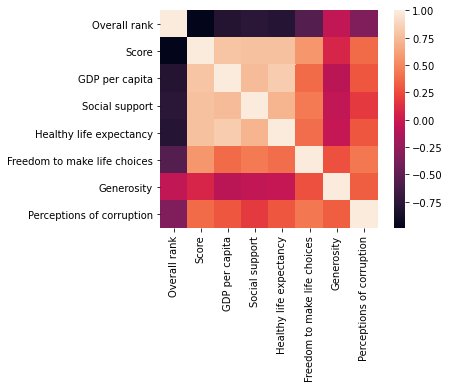
\includegraphics[scale=0.40]{heatmap.png}
\caption{Heatmap}
\end{figure}

\begin{figure}[htp]
\centering
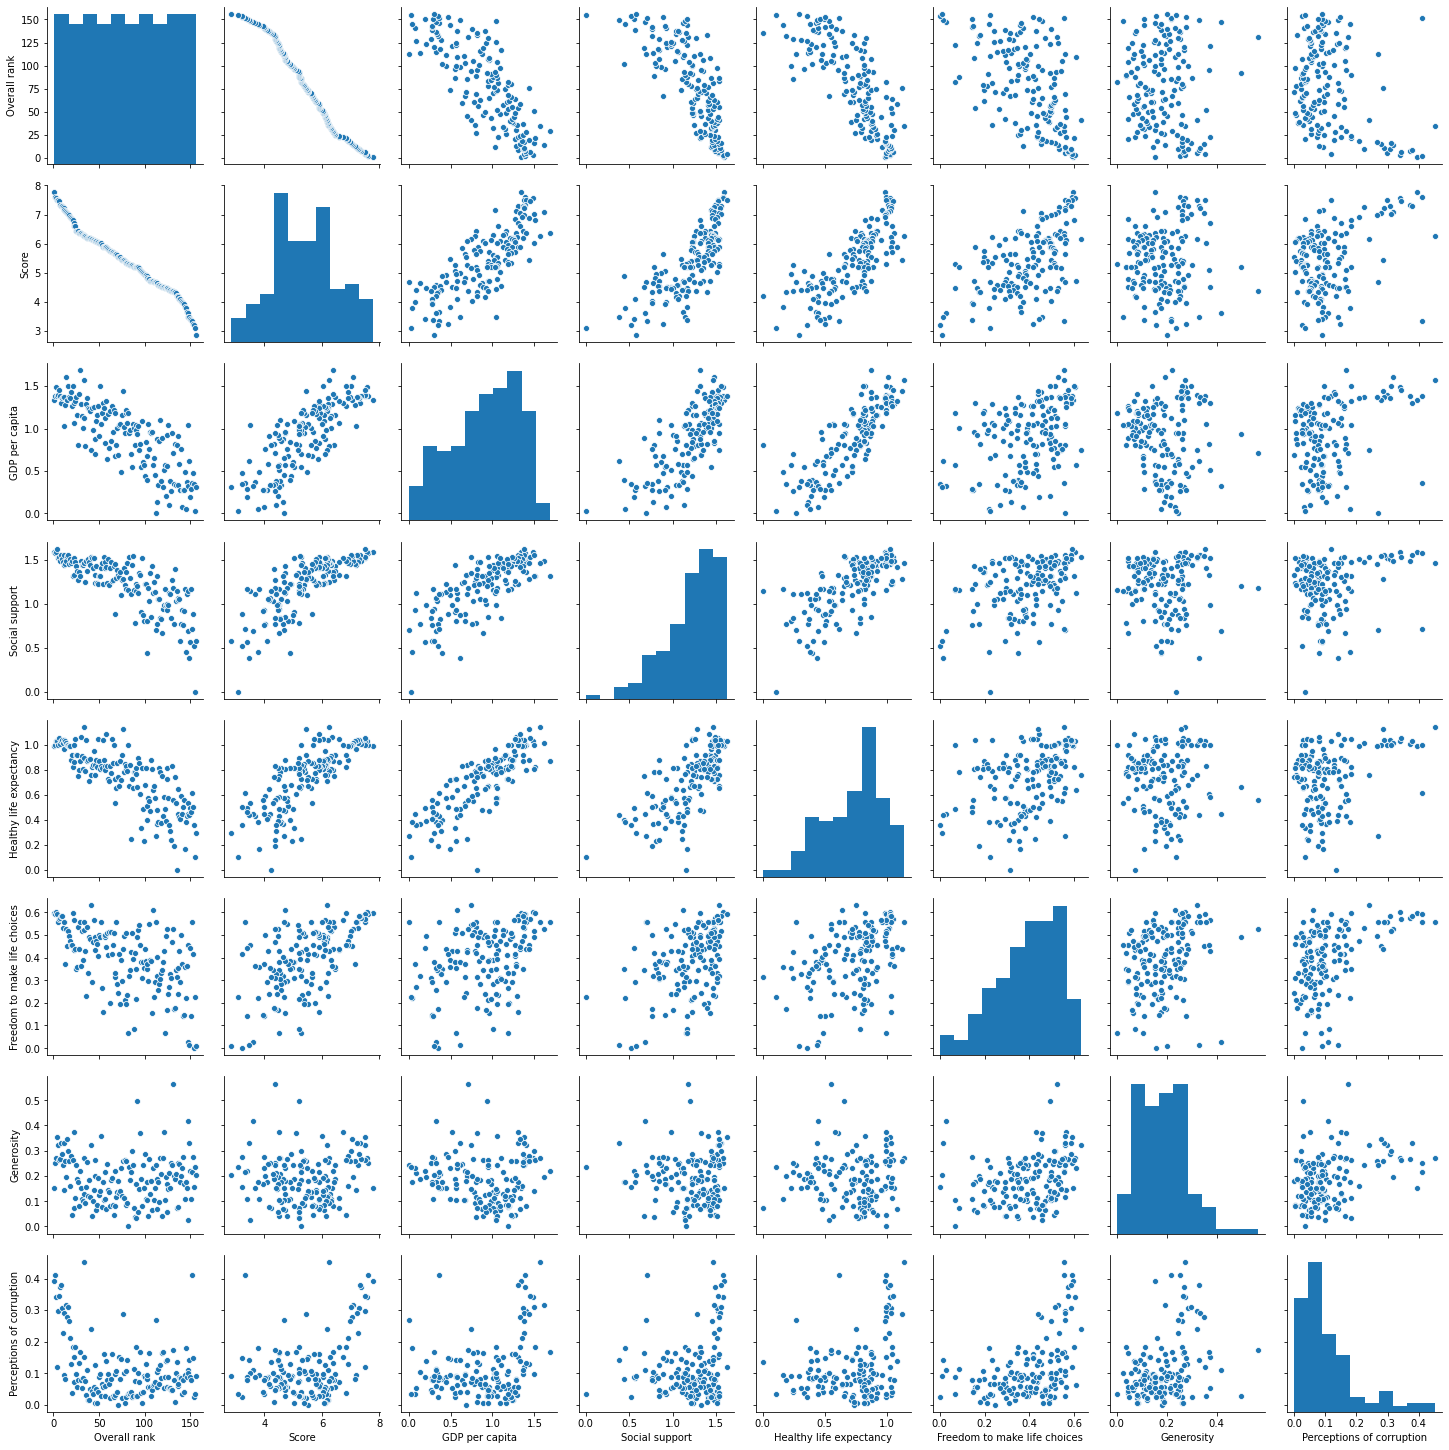
\includegraphics[scale=0.15]{pairplot.png}
\caption{Plotting pairwise relationships in the dataset}
\end{figure}

\clearpage

\begin{figure}[htp]
\centering
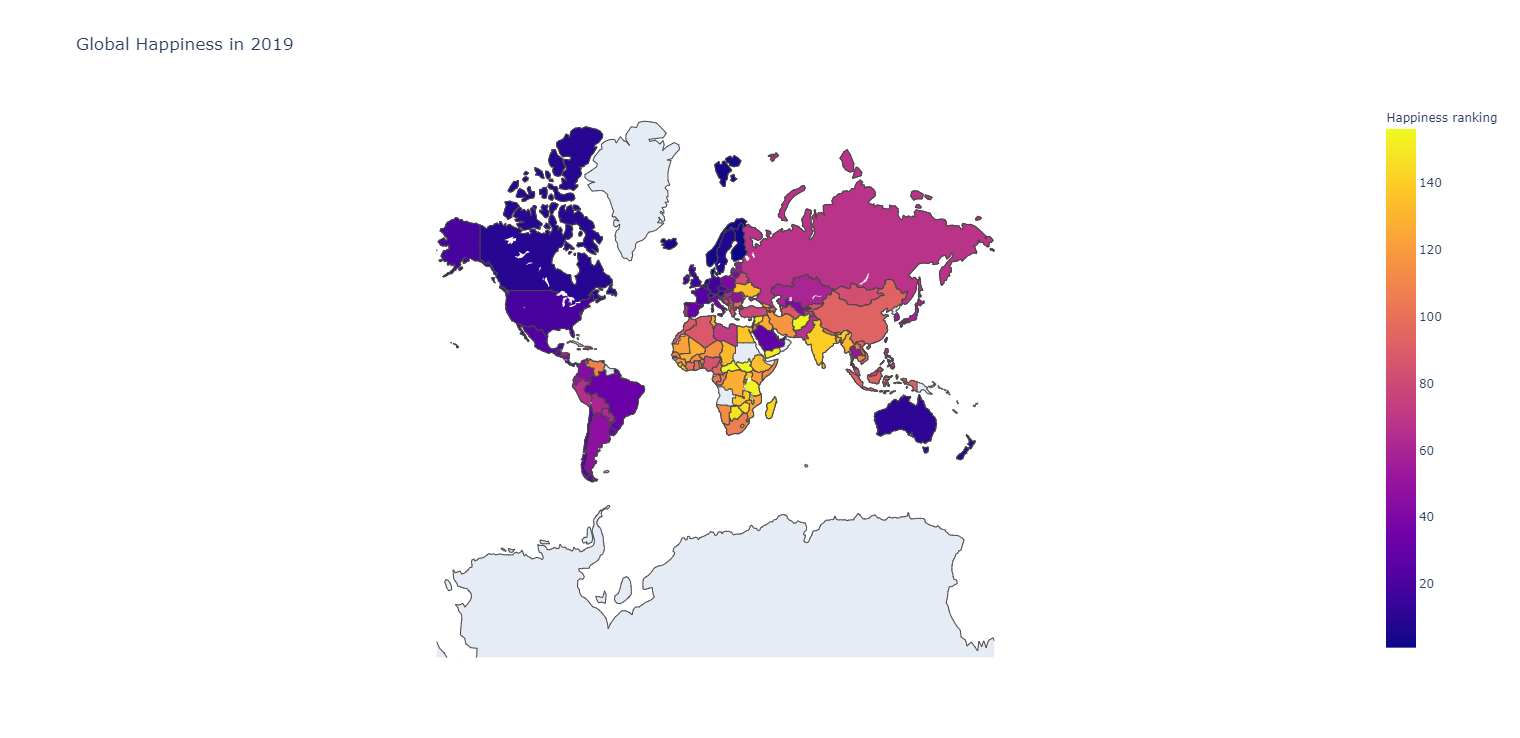
\includegraphics[scale=0.30]{globalmap.png}
\caption{Happiness ranking of countries}
\end{figure}


\begin{figure}[htp]
\centering
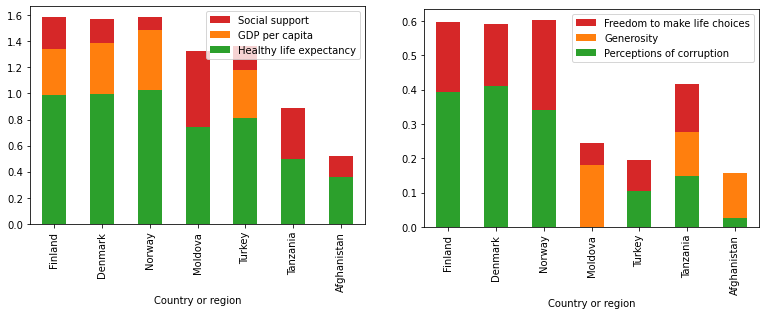
\includegraphics[scale=0.70]{country.png}
\caption{Comparison of countries according to 6 features}
\end{figure}
\clearpage

\begin{figure}[htp]
\centering
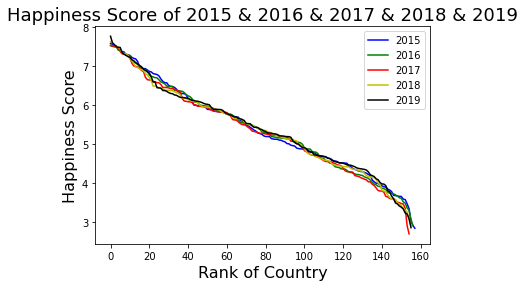
\includegraphics[scale=0.60]{score.png}
\caption{Happiness Score 2015\&2016\&2017\&2018\%2019}
\end{figure}

\begin{figure}[htp]
\centering
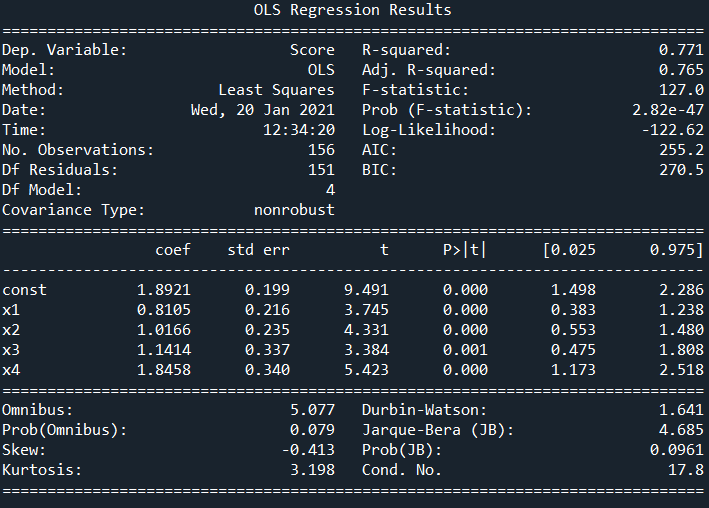
\includegraphics[scale=0.60]{ols.png}
\caption{Last output of OLS Regression Results}
\end{figure}
\clearpage

\begin{figure}[htp]
\centering
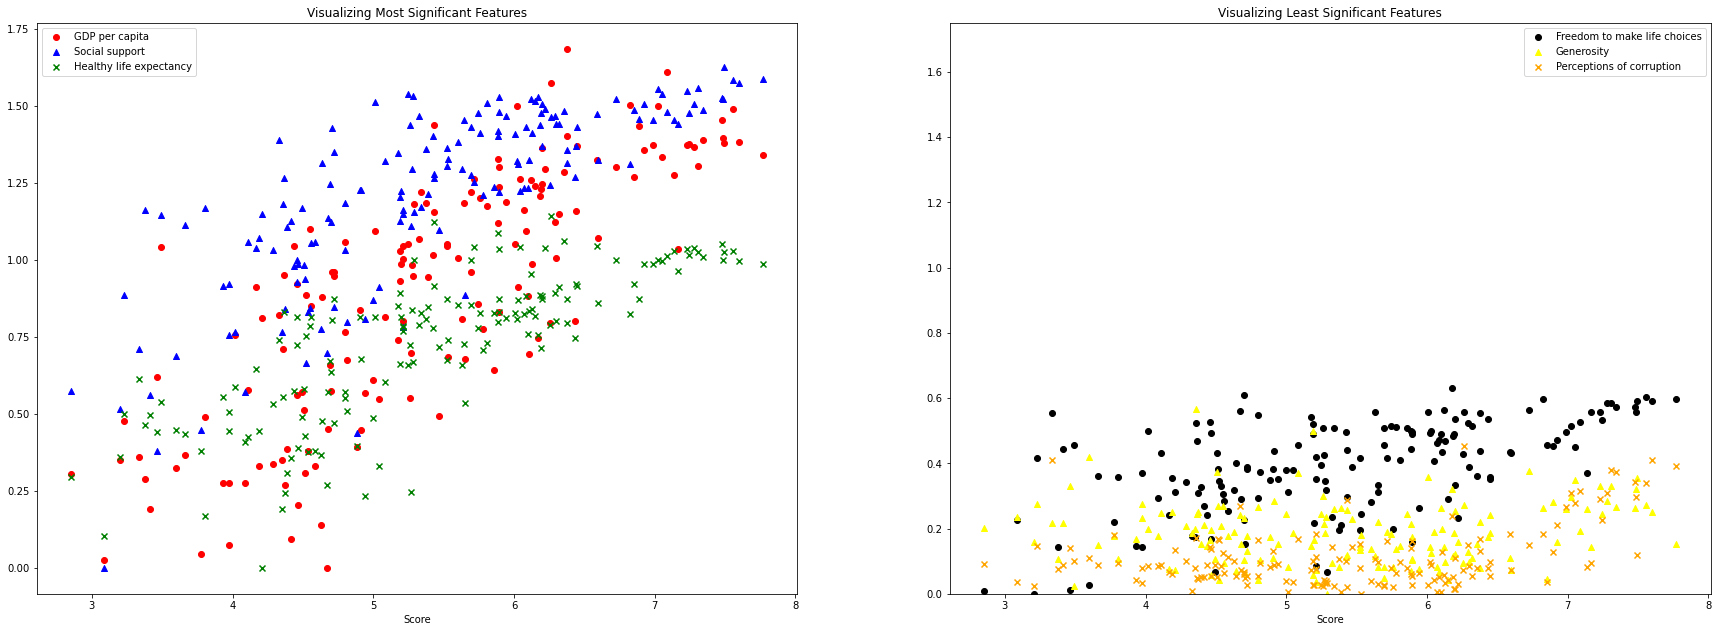
\includegraphics[scale=0.25]{features.png}
\caption{Visualizing Features}
\end{figure}

\begin{figure}[htp]
\centering
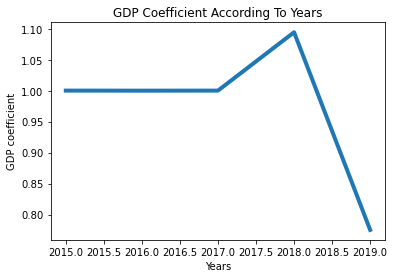
\includegraphics[scale=0.50]{gdp.png}
\caption{GDP coefficient according to years}
\end{figure}

\begin{figure}[htp]
\centering
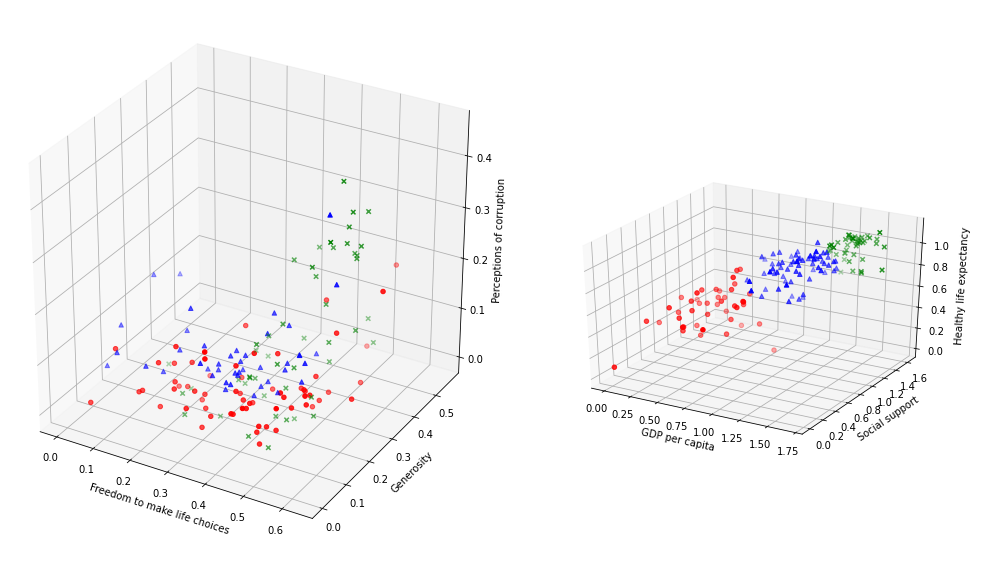
\includegraphics[scale=0.50]{clustering3.png}
\caption{Clustering}
\end{figure}

\begin{figure}[htp]
\centering
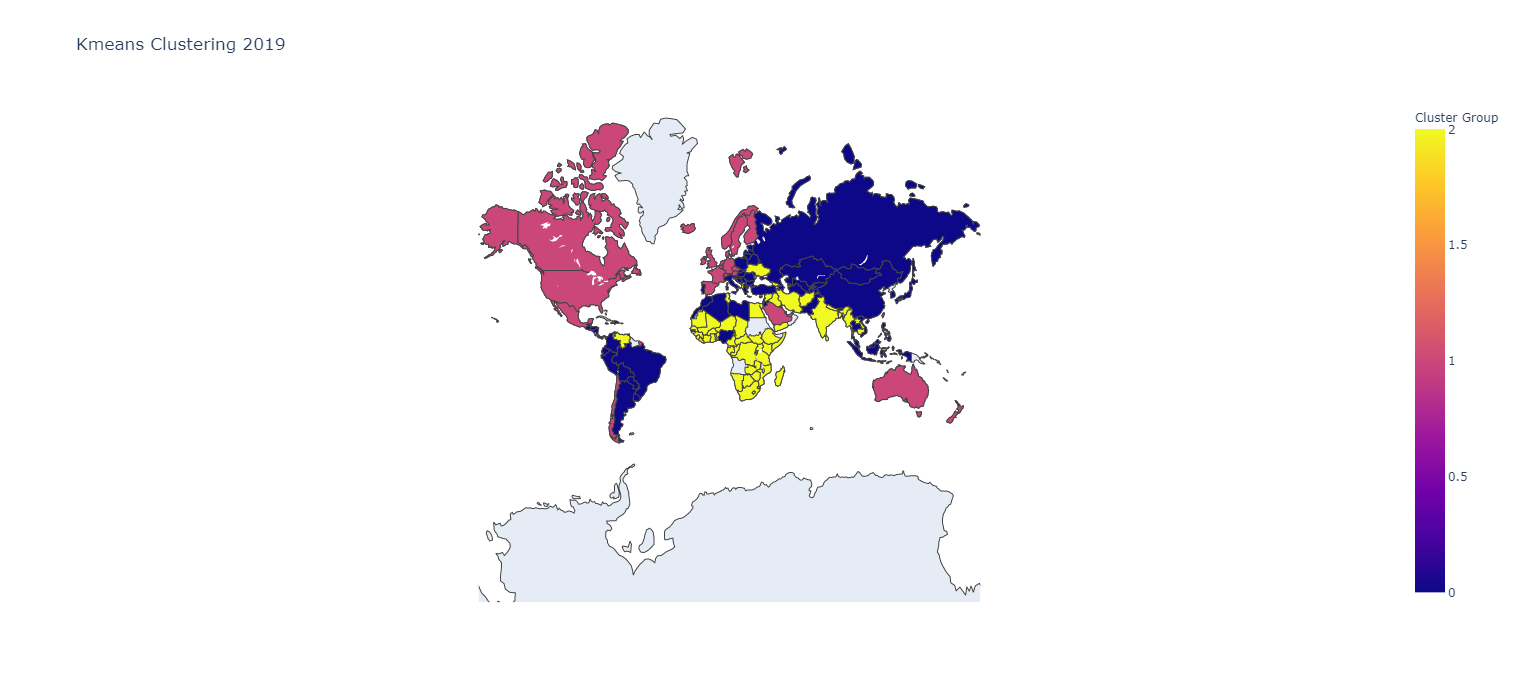
\includegraphics[scale=0.30]{clusteringmap.png}
\caption{Kmeans Clustering 2019}
\end{figure}

\begin{figure}[htp]
\centering
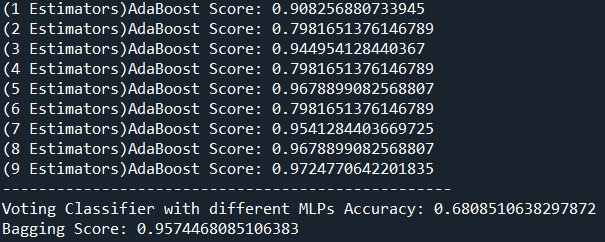
\includegraphics[scale=0.60]{ensembleLearning.png}
\caption{Ensemble learning scores}
\end{figure}






\clearpage
\section{Conclusion}
As a result, using Figure 2, Figure 3, and Figure 8, we showed that the features that most affected our data set were GDP per capita, social support, and healthy life expectancy. We checked and verified this information statistically using the backward elimination method. In other words, we have revealed the country characteristics that are necessary for people in a country to be happy and to live a good life.

Apart from that, in Figure 4, we visualized our data set on the map so that the happiness rankings of the countries appear as a whole and our data can be understood more easily.

Later, in Figure 5, we compared the 3 happiest countries with the moderate and less happy countries, and as a result of this comparison, we saw that the most important feature in the 3 happiest countries was healthy life expectancy. In addition, we observed that the least common feature in these 3 countries is generosity. The common feature of the most unhappy countries was that GDP per capita values were very low. The countries which have middle happines score (such as Turkey) might seem that their most important features are good, but the low scores in the least affecting features has led to remain in their mid status.

In Figure 6, we have shown that the happiness score corresponding to each country's rankings has not changed much over the years.

In the linear regression part of our project, we first estimated the 2019 data set from the 2018 data set. We used the R2 score to measure the accuracy of our model. As seen in Figure 1, this value came around "0.77". This showed us the accuracy of our model. (Note: The value of R2 when the model predicts 100\% correct is 1.) This trained model can also be used to predict future years.

In the second part on linear regression, we visualized the effect of GDP per capita over all years. As can be seen from Figure 9, while GDP per capita value was given a stable importance before 2018, in 2018, a lot of attention was paid to GDP per capita value. In 2019, this importance has decreased even more than it was in 2015, 2016, 2017. This has shown us that the factors that people care about may change over the years and lead to changes in the ranking of happiness.

Regarding the clustering part, we first clustered our data set in Figure 10 according to the most effective and least effective features. As a result, we found that GDP per capita, healthy life expectancy, social support features were in a linear correlation. We have seen that other features are not correlated in the same way and are irregular in such a way that no meaning can be made.

Finally, we have shown the countries in 3 different groups by using visualization on the map again in Figure 11. The first of these groups belongs to the happiest countries, the other to the countries of medium happiness, and the last to the unhappy countries.
Thanks to this visualization, we analyzed our data more easily, showed in which continent there are more happy people and the welfare level of the countries.

Some of the models we trained with the AdaBoost objects we created had scores of 95\% and some 79\%. Our model, which we trained with Voting Classifier, or MLPs, showed a worse result compared to other algorithms and remained around 68\%. Our model, which we trained with bagging, showed a very good success with a score of 95\%.
Considering these results, we have seen that it would be better to use Boosting or Bagging when such data is encountered. Thanks to these algorithms, we achieved very good results using weak learners and we did unsupervised learning by creating our own classes with clustering.

\nocite{*}

\end{document}


